\documentclass{sig-alternate}

\usepackage{enumitem}
\usepackage{framed}
\usepackage{listings}
\usepackage{amstext}
\usepackage{amstext}
\usepackage{pdfpages}
\usepackage{alltt}
\usepackage{epstopdf}
\usepackage{xspace,colortbl}
\usepackage[USenglish]{babel}
\usepackage{multirow}
\usepackage{url}
\usepackage{subfigure}
\usepackage{graphicx}
\usepackage{amssymb}
\usepackage{fmtcount}
\usepackage{amsfonts}
\usepackage{xspace}
\usepackage{amsmath}
\usepackage{multirow}
\usepackage[mathscr]{eucal}
%\usepackage{psfrag}
\usepackage{colortbl}
\usepackage{bm}
\usepackage[nospace]{cite}


\usepackage[algoruled,vlined,linesnumbered]{algorithm2e}
\usepackage{xcolor}
\newcommand\mycommfont[1]{\scriptsize\ttfamily\textcolor{blue}{#1}}
\SetCommentSty{mycommfont}
\SetKwFor{ParForAll}{for}{do in parallel}{end}
\SetKw{WaitUntil}{wait until}


\lstset{basicstyle=\scriptsize,breaklines=true}

\linespread{0.94}%

\makeatletter
\def\@copyrightspace{\relax}
\makeatother

\begin{document}

\setlength{\belowdisplayskip}{2pt} \setlength{\belowdisplayshortskip}{2pt}
\setlength{\abovedisplayskip}{2pt} \setlength{\abovedisplayshortskip}{2pt}
\setlength{\belowcaptionskip}{-8pt}
\selectfont

\newtheorem{theorem}{Theorem}
\newtheorem{example}{Example}
\newtheorem{definition}{Definition}
\newtheorem{proposition}{Proposition}
\newtheorem{lemma}{Lemma}
\newtheorem{corollary}{Corollary}

\newcommand{\cond}{\textrm{Cond}\xspace}
\newcommand{\dataset}{data set\xspace}
\newcommand{\datasets}{data sets\xspace}
\newcommand{\spview}{\textsf{SPView}\xspace}
\newcommand{\fjview}{\textsf{FJView}\xspace}
\newcommand{\aggview}{\textsf{AggView}\xspace}
\newcommand{\hashfunc}[1]{\textsf{hashfunc}(#1)\xspace}

\newcommand{\avgfunc}{\ensuremath{\texttt{avg} }\xspace}
\newcommand{\maxfunc}{\ensuremath{\texttt{max} }\xspace}
\newcommand{\minfunc}{\ensuremath{\texttt{min} }\xspace}
\newcommand{\histfunc}{\ensuremath{\texttt{histogram\_numeric} }\xspace}
\newcommand{\countfunc}{\ensuremath{\texttt{count}}\xspace}
\newcommand{\sumfunc}{\ensuremath{\texttt{sum} }\xspace}
\newcommand{\varfunc}{\ensuremath{\texttt{var} }\xspace}
\newcommand{\covfunc}{\ensuremath{\texttt{cov} }\xspace}
\newcommand{\corrfunc}{\ensuremath{\texttt{corr} }\xspace}
\newcommand{\medfunc}{\ensuremath{\texttt{median} }\xspace}
\newcommand{\percfunc}{\ensuremath{\texttt{percentile} }\xspace}
\newcommand{\havingfunc}{\ensuremath{\texttt{HAVING} }\xspace}
\newcommand{\ratio}{\ensuremath{\rho }\xspace}


\newcommand{\scp}{\textbf{SampleCleanPipeline}\xspace}
\newcommand{\sca}{\textbf{SampleCleanAlgorithm}\xspace}


\newcommand{\insertion}{\ensuremath{\texttt{INSERT} }\xspace}
\newcommand{\update}{\ensuremath{\texttt{UPDATE} }\xspace}
\newcommand{\delete}{\ensuremath{\texttt{DELETE} }\xspace}


\newcommand{\tbl}[1]{\textsf{#1}\xspace}
\newcommand{\field}[1]{\textsf{#1}\xspace}
\newcommand{\cost}{\textrm{cost}\xspace}
\newcommand{\ans}{\textsf{ans}\xspace}
\newcommand{\dans}{\Delta\textsf{ans}\xspace}
\newcommand{\cqp}{correction query processing\xspace}
\newcommand{\Cqp}{Correction query processing\xspace}

\newcommand{\reminder}[1]{{{\textcolor{magenta}{\{\{\bf #1\}\}}}\xspace}}
\newcommand{\specialcell}[2][c]{%
  \begin{tabular}[#1]{@{}c@{}}#2\end{tabular}}

\def\ojoin{\setbox0=\hbox{$\bowtie$}%
  \rule[-.02ex]{.25em}{.4pt}\llap{\rule[\ht0]{.25em}{.4pt}}}
\def\leftouterjoin{\mathbin{\ojoin\mkern-5.8mu\bowtie}}
\def\rightouterjoin{\mathbin{\bowtie\mkern-5.8mu\ojoin}}
\def\fullouterjoin{\mathbin{\ojoin\mkern-5.8mu\bowtie\mkern-5.8mu\ojoin}}

%\newcommand{\reminder}[1] {}
\pagestyle{plain}

\title{A Monte-Carlo Approach For Robust Execution of Heuristic Entity Resolution Pipelines}

\maketitle


\vspace{-1em}

\begin{abstract}
\reminder{TODO}
\end{abstract}


\section{Introduction}
Large datasets can be prone to error \cite{Gartner}, and data cleaning has been studied to mitigate query error on dirty data \cite{dasu2003exploratory, mayfield2010eracer, openrefine, wrangler, DBLP:conf/sigmod/DallachiesaEEEIOT13, DBLP:conf/pervasive/JefferyAFHW06}.
An important subclass of data cleaning problems are Entity Resolution (ER) problems which have had much research interest both historically and recently. \cite{DBLP:journals/pvldb/KopckeTR10, conf/dmkd/MongeE97, conf/sigmod/WhangMKTG09, conf/acl/FinkelM08, conf/sigmod/WangLF12, Fellegi1969, conf/sigmod/ArasuGK10, DBLP:journals/tkde/ElmagarmidIV07, journals/tkde/Christen11, getoor2005link}
In these problems, for every record we want to find a single canonical mapping between the record and a real-world entity.
This includes regularizing representations, removal of duplicate records, and removal of irrelevant records.

A popular theoretical model for ER is the functional dependency model.
The concept of a functional dependency has been well studied in the database literature 
and was proposed by Codd in 1974 \cite{codd1974recent}.
Recent work explores encoding ER primitives as types of functional dependencies called Conditional Functional Dependencies (CFD) \cite{bertossi2013data, fan2014interaction, fan2008conditional}.
These are basically rules that encode unsatisfied constraints based on expert input (i.e NY == New York) and the data cleaning algorithm iterates until these constraints are satisfied.
As this formulation fits nicely into a Satisfiability-like framework, many theoretical insights have naturally followed such determining the minimal sequence of data changes to satisfy all of the constraints is coNP-Hard. \reminder{SK: todo clarify section}

As the coNP-Hard result suggests, while this model gives insights into what types of errors occur in a dataset, there is a challenge of efficiently repairing the errors (i.e. enforcing the constraints).
Bertossi et al. \cite{bertossi2013data} found that a lattice data structure could be used to a find PTIME iterative algorithm for ER problems with only ``matching" dependencies.
Wang et al. \cite{wang2014towards} extended the CFD framework with ``fixing" rules; rules that also prescribed fixes which as in Bertossi et al. makes the cleaning algorithms faster and more reliable.

A key assumption of the functional depedency work in data cleaning has been \emph{infallible} rules.
However, in practice, this is rarely the case.
Large datasets are often pre-processed with chains of heuristic data cleaning operations each with their own precision and recall characteristics as in ETL tools \cite{herzog2007data}.
Furthermore, increasingly data cleaning is part of a larger pipeline including streaming, machine learning, or exploratory data analysis.
In this setting, semantics on partial or sampled results are important, and the CFD model may not be appropriate to describe these applications.

In this work, we explore robust execution of \emph{pipelines} of data cleaning operations with an application to ER.
In contrast to prior work, we formalize ER as an algebra over relations as opposed to constraints on tuples in those relations.
A key piece of this work is a data structure we call a \emph{proposal} which propagates an augemnted intermediate state of the pipeline mitigating some times of errors.
We show that in the case where our operations are \emph{infallible}, our formalization naturally leads to the algorithm proposed by Bertossi et al., and exactly the same result with a connected components algorithm over a graph of linked tuples.
However, the connected components version is robust to transitivity errors in the rules which correspond to missing edges in the graph.
We then devise an alternative to the connected components, accounting for spurious edges, using correlation clustering which seperates the graph into components that are approximately cliques.
Finally, we merge proposal data structures from different executions allowing us to try different permutations of the ER pipeline and take a consensus of their results.










\section{Background and Main Ideas}

This section describes the key idea of SampleClean, namely, that data cleaning can be integrated with approximate query processing leading to bounded approximations of clean query results for a fraction of the cleaning cost.

\iffalse
\subsection{Data Cleaning is Often Expensive}
A number of surveys report that data cleaning is one of the most time consuming steps \cite{kandel2012enterprise, nytimes}.
Data cleaning frameworks have been recently proposed to address the problem of corrupted data at scale\cite{khayyat2015bigdansing, chu2015katara, sampleclean}.
As errors can be domain- or dataset-specific, data cleaning is an inherently human-driven process and can require a significant amount of developer effort in writing software or rules to fix the corruption.
Automated fixes may not be reliable and can require human confirmation \cite{DBLP:journals/pvldb/YakoutENOI11}.
One way to scale up human computation is crowdsourcing which has shown recent success in entity resolution and value filling \cite{gokhale2014corleone, park2014crowdfill, sampleclean,chu2015katara}.
However, crowdsourcing comes with the costs of significant additional latency (orders of magnitude slower than data processing) and the overhead of managing human workers.
\fi

\subsection{Traditional Approximate Query Processing}
A number of approximation schemes have been proposed including using Sampling, Wavelets, Sketching, and Hashing (see Cormode et al. for a survey \cite{DBLP:journals/ftdb/CormodeGHJ12}).
This article focuses on Sampling-based approximations and we will use the term AQP to refer to such systems (e.g., BlinkDB\cite{DBLP:conf/eurosys/AgarwalMPMMS13}).
Sampling-based approximate query processing is a powerful technique that allows for fast approximate results on large datasets. 
It has been well studied in the database community since the 1990s~\cite{DBLP:conf/sigmod/HellersteinHW97,DBLP:conf/sigmod/AcharyaGPR99,DBLP:conf/icde/OlkenR92, OlkenR86}, and methods such as BlinkDB~\cite{DBLP:conf/eurosys/AgarwalMPMMS13} have drawn renewed attention in recent big data research. 
An important aspect of this work is confidence intervals, as many types of aggregates can be bounded with techniques such as concentration inequalities (e.g., Hoeffding bounds), large-deviation inequalities (e.g., Central Limit Theorem), or empirically (e.g., Bootstrap). 
Suppose, there is a relation $R$ and a uniform sample $S$.
AQP applies a query $Q$ to $S$ (possibly with some scaling $c$) to return an estimate: 
\[
Q(R) \approx est = c \cdot Q(S)
\]

Traditionally, AQP sacrifices accuracy due to sampling for improved query latency.
However in AQP, the bounds on $est$ assume that the only source of error is approximation error introduced by sampling, however, the data itself may contain errors which could also affect query results.
When the data itself is erroneous, a query result on the full data--let alone a sample, will be incorrect.
The main argument for SampleClean is that when data errors significantly affect query results,
sampling can be combined with data cleaning to actually improve accuracy.
This leads to a counter-intuitive result where it is possible that a query on a cleaned sample of data is more accurate than a query on the entire dirty data.

\iffalse
\subsection{Exploiting Application Structure}

\jn{It's a little too early to present the content of this section before showing the big idea. I would suggest to put it either to the end of Sec 2 or the end of Sec 3. }

SampleClean applies sample to clean $k\ll N$ rows in a database to address the time-scale mismatch between the analytics application (e.g., SQL query, Machine Learning, Materialized View) and data cleaning.
An important aspect of this project is how the structure and semantics of that application can be used to prioritize and budget data cleaning.
A database only needs to be sufficiently clean for the requirements of the subsequent analytics--and the key insight from AQP being that aggregates are tolerant to approximation.

In the initial SampleClean work, we restricted the allowed aggregate queries to \sumfunc, \countfunc, and \avgfunc with predicates and group by clauses.
In the two subsequent projects, View Cleaning and ActiveClean, we expanded the scope and the semantics of the application. 
The View Cleaning problem explores data cleaning and general aggregates on derived relations with known view definitions.
We can exploit view definition to query just as much of the base data as needed to accurately answer the aggregate query for a fixed budget.
In fact, we showed that any aggregate (beyond \sumfunc, \countfunc, and \avgfunc) that could be estimated with AQP\cite{agarwalknowing}, could be answered estimated with the View Cleaning framework.
ActiveClean generalizes the initial work on \sumfunc, \countfunc, and \avgfunc to higher-dimensional aggregates.
We defined a class of analytics called Convex Data Analytics, and show how the convex structure of the analytics can be used to guide and prioritize data cleaning.
\fi

\subsection{Approximate Query Processing on Dirty Data}


\subsubsection{Two Sources of Errors: Sampling Error and Data Error}
If $R$ is dirty, then there is a true relation $R_{clean}$.
\[
Q(R_{clean}) \ne Q(R) \approx est = c \cdot Q(S)
\]
The error in $est$ has two components: error due to sampling $\epsilon_s$ and error due to the difference with the cleaned relation $\epsilon_c = Q(R_{clean}) - Q(R)$:
\[
\mid Q(R_{clean}) - est \mid \le \epsilon_s + \epsilon_c
\]

While they are both forms of query result error, $\epsilon_s$ and $\epsilon_c$ are very different quantities.
$\epsilon_s$ is a random variable due to the sampling, and different samples would result in different realizations of $\epsilon_s$.
As a random variable introduced by sampling, $\epsilon_s$ can be bounded by a variety of techniques as a function of the sample size.
On the other hand, $\epsilon_c$ is deterministic, and by definition is an unknown quantity until all the data is cleaned.
Thus, the bounds returned by a typical AQP framework on dirty data would neglect $\epsilon_c$.

It is possible that $R_{clean} \ne R$ but $\epsilon_c=0$.
Consider a \sumfunc query on the relation $R(a)$, where $a$ is a numerical attribute.
If half of the rows in $R$ are corrupted with $+1$ and the other half are corrupted with $-1$, then $Q(R_{clean}) = Q(R)$.
The interesting problem is when there are \emph{systematic errors}\cite{taylor1982introduction} i.e., $\mid \epsilon_c \mid > 0$. 
In other words, the corruption that is correlated with the data, e.g., where every record is corrupted with a $+1$.

\subsubsection{Key Idea I: Direct Estimate vs. Correction}
The key quantity of interest is $\epsilon_c$, and to be able to bound
a query result on dirty data, requires that $\epsilon_c$ is 0 or bound $\epsilon_c$.

\vspace{0.5em}
\noindent\textbf{Direct Estimate: } This technique is a direct extension of AQP to handle data cleaning. A set of $k$ rows is sampled uniformly at random from the dirty relation $R$ resulting in a sample $S$. Data cleaning is applied to the sample $S$ resulting in $S_{clean}$.
Data cleaning and sampling may change the statistical and scaling properties of the query $Q$, so $Q$ may have to be re-written to a query $\widehat{Q}$. $\widehat{Q}$ is applied to the sample $S_{clean}$ and the result is returned. 
There are a couple of important points to note about this techniques.
First, as in AQP, the direct estimate only processes a sample of data.
Next, since it processes a cleaned sample of data, at no point is there a dependence on the dirty data.
As we will show later in the article, the direct estimate returns a result whose accuracy is independent of the magnitude or rate of data error. 
One way to think about this technique is that it ensures $\epsilon_c = 0$ within the sample.

\vspace{0.5em}
\noindent\textbf{Correction: } The direct estimate suffers a subtle drawback. Suppose, there are relatively few errors in the data. The errors introduced by sampling may dominate any error reductions due to data cleaning. As an alternative, we can try to estimate $\epsilon_c$. A set of $k$ rows is sampled uniformly at random from the dirty relation $R$ resulting in a sample $S$. Data cleaning is applied to the sample $S$ resulting in $S_{clean}$. 
The difference in applying $\widehat{Q}$ to S and $\widehat{Q}$ to $S_{clean}$ gives an estimate of $\epsilon_c$. 
The interpretation of this estimate is a correction to the query result on the full dirty data.
In contrast to the direct estimate, this technique requires processing the entire dirty data (but only cleaning a sample).
However, as we will later show, if errors are rare this technique gives significantly improved accuracy over the direct estimates.

\subsubsection{Key Idea II: Sampling to Improve Accuracy}
%A small sample of clean data can improve query accuracy.
Figure \ref{fig:est2} plots error as a function of the cleaned sample size on a corrupted TPCH dataset for a direct estimate, correction, and AllDirty (query on the full dirty data).
In both cases, there is a break-even point (in terms of number of cleaned samples) when the data cleaning has mitigated more data error than the approximation error introduced by sampling.
After this point, SampleClean improves query accuracy in comparison to AllDirty.
When errors are relatively rare (5\% corruption rate), the correction is more accurate. 
When errors are more significant (50\% corruption rate), the direct estimate is more accurate.
Note that the direct estimate returns results of the same accuracy regardless of the corruption rate. 

\begin{SCfigure}
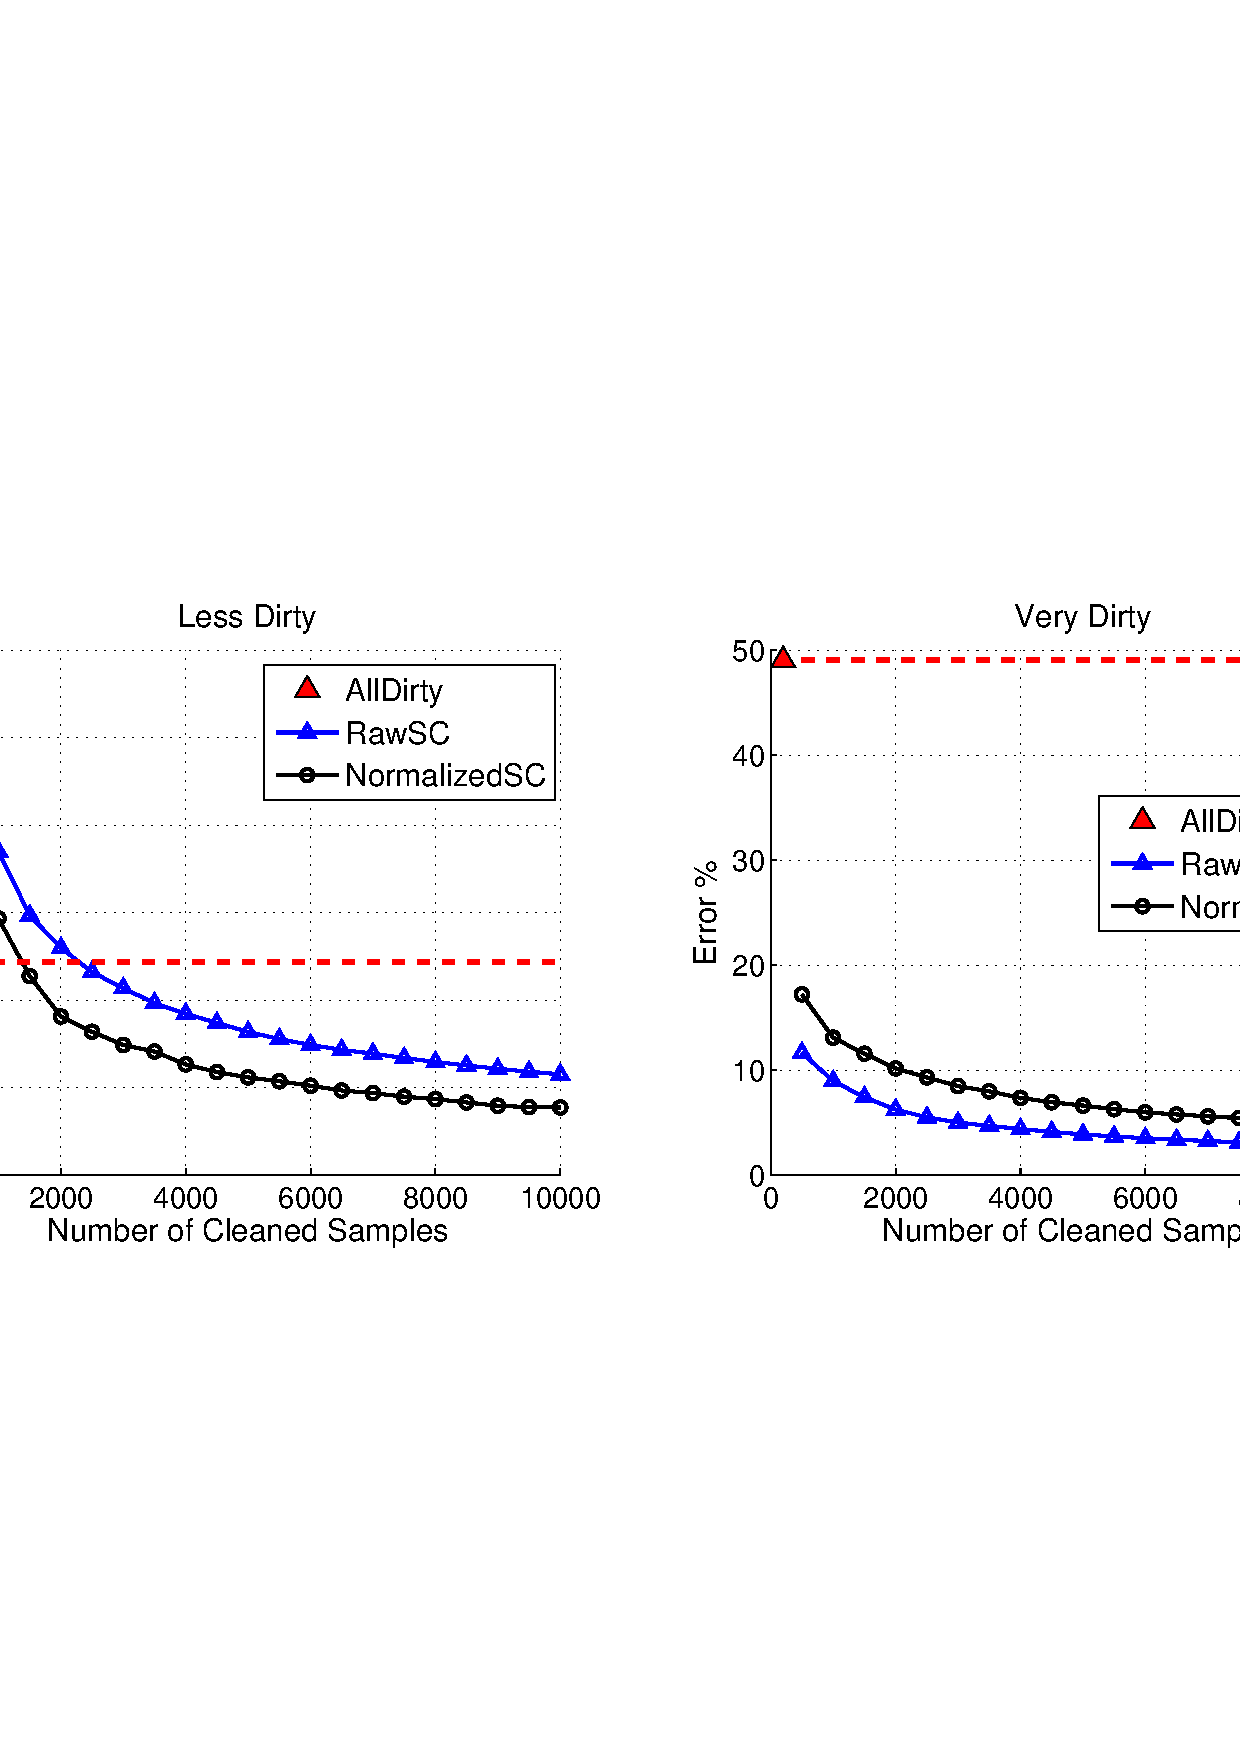
\includegraphics[width=.6\columnwidth]{figs/allerror-samplesize.pdf}
\caption{Comparison of the convergence of the methods on two TPC-H datasets of 6M tuples with simulated errors 50\% error and 5\% error. On the dataset with larger errors, the direct estimate gives a narrower confidence interval, and on the other the correction is more accurate. \label{fig:est2}}
\end{SCfigure}




\section{Proposals}
We first look at subproblem relevant to the pipeline optimization; how do we represent the relationships 
between tuples in these entity resolution tasks.
We call this intermediate data structure a proposal since metaphorically the data cleaning operations propose changes.
The execution engine then takes this proposal and formulates an actionable execution plan based on the proposal actually apply the changes.

The solution will be to break apart the ER operators in the previous section and represent their operations
as a graph.
In this section, we describe this procedure for a single given pipeline.
Then, we discuss how to merge different proposals.

\subsection{Building Proposals}
We re-define entity resolution in terms of what we call \emph{proposal operations}.
That is instead of making a change, the operation proposes a candidate change.
By exposing this intermediate state rather than immediate applying changes, we can relax some of the assumptions we made
in the previous section when formalizing entity resolution.

First, $\delta$ operations need not execute one-to-one merges.
We can propose a set of candidate merges e.g. row1 one is linked to row2 and row3.
Similarly, with $\kappa$ operations we can propose a set of possible transformations e.g. if my attribute is a comma separated string value, the relevant data is either in 1st or 2nd field.
We can defer enforcing correctness to when the proposal is actually executed.
One way to think about this approach is that we are building a probabilistic database on a deterministic database and lazily marginalizing the distributions at execution time [cite].

\begin{definition} Entity Resolution Proposals. 
Proposal operations are functional operations on a weighted graph $G=(V,E,W(e),M(v))$ with edge weights $W(e)$ and a multiplicity function $M(v)$ for each vertex. 
Records in the database are represented as vertices, and proposed corrections/merges are represented as edges.
\begin{itemize}
\item Correct $\kappa(G,a_{1})$ For every $v \in V$, let $v'$ be the corrected version of $v$. We add $v'$ to $V$ if it does not exist and we draw an edge between $v$ and $v'$ with weight $w$ where a larger $w$ indicates increased confidence. If it already exists, we increment the multiplicty counter for $v'$. If $v$ has multiple possible corrected versions, repeat for all.
\item Deduplication $\delta(G)$ For every $v \in V$, draw an edge starting at $v$ to represent merging two records with weight $w$ where a larger $w$ indicates increased confidence. If it has multiple possible merges, draw edges for all.
\end{itemize}
%Like before, we constrain that $\kappa$ and $\delta$ are consistent; that is given two records that are identical on the projection their operation is identical.
\end{definition}

The end of a given pipeline will be a graph $G$. 
This graph structure is a generalization of the graph structure discussed in entity resolution [cite]; i.e. the graph in an open world model.

\subsection{Proposal API}
\reminder{TODO}

\subsection{Benefits from this Data Structure}
We list out some of the benefits of this data structure and what we can do with proposals that was not previously possible in pipeline of ``off-the-shelf" entity resolution components. First, proposals give a natural way to represent uncertainty using weighted edges. They also subsume deterministic algorithms as we can represent a tree of merges with uniform weights. It is true that internally, many ER algorithms use a similar construction, however, by building a single, unfied data structure to represent both $\kappa$ and $\delta$ operations, we can propagate the data structure through a pipeline of reusable components. 

The second benefit is a representation of history. 
By representing the $\kappa$ operations in the data structure, we do not lose history when we apply an operation.
For example, an operation might be correct for 80\% of records and give incorrect results for the last 20\%, and the data structure gives us a natural way to interface with previously correct results.

The practical implications of this structure are interesting. 
For example, in ER pipelines, we often have to make many decisions up front such as what string tokenizer to use, how to threshold heuristics, or how dates should be formatted.
In this model, with the proposal structure, we argue why not try all of them.
Obviously there is a trade-off space between ER accuracy and performance, and we will discuss that more in the next section.

\subsection{Proposal Overhead}
The proposal framework introduces overhead as the graph $G$ is much larger in terms of both edges and vertices than typically considered in graph based ER tasks. 
This warrants new algorithms to process this larger graph.
If $p$ is the number of steps in the pipeline, and $k$ is the average number of candidates $O(p^2k^2+V^2)$.
\reminder{TODO}

\subsection{Algebra Over Proposals}
Given two different proposals $G_1$ and $G_2$, we can define a merge operations to make them a single proposal.
\reminder{TODO}


\section{Efficiency With Sampling}\label{dist-samp}
The model update received a sample with probabilities $p(\cdot)$.
For any distribution where  $p(\cdot) > 0$, we can preserve correctness.
\sys uses a sampling algorithm that selects the most valuable records to clean with higher probability. 

\subsection{Oracle Sampling Problem}
Recall that the convergence rate of an SGD algorithm is bounded by $\sigma^2$ which is the variance of the gradient.
Intuitively, the variance measures how accurately the gradient is estimated from a uniform sample.
Other sampling distributions, while preserving the sample expected value, may have a lower variance.
Thus, the oracle sampling problem is defined as a search over sampling distributions to find the minimum variance sampling distribution.

\begin{definition}[Oracle Sampling Problem]
Given a set of candidate dirty data $R_{dirty}$, $\forall r \in R_{dirty}$ find sampling probabilities $p(r)$ such that over all samples $S$ of size $k$ it minimizes:
\[
\mathbb{E}(\|g_S - g^*\|^2)
\]
\end{definition}
It can be shown that the optimal distribution over records in $R_{dirty}$ is probabilities proportional to:
\[
p_i \propto \|\nabla\phi(x^{(c)}_i,y^{(c)}_i,\theta^{(t)})\|
\]
We provide proofs and theoretical justification in appendix, but intuitively, records with higher gradients should be sampled with higher probability as they affect the update more significantly.
However, this cannot exclude records with lower gradients as that would induce a bias hurting convergence.
The problem is that this optimal distribution leads to a chicken-and-egg problem:
the optimal sampling distribution requires knowing $(x^{(c)}_i,y^{(c)}_i)$, however, cleaning is required to know those values.

\subsection{Dirty Gradient Solution}
Such an oracle does not exist, and one solution is to use the gradient w.r.t to the dirty data:
\[
p_i \propto \|\nabla\phi(x^{(d)}_i,y^{(d)}_i,\theta^{(t)})\|
\]
It turns out that this solution works reasonably well in practice on our experimental datasets and has been studied in Machine Learning as the Expected Gradient Length heuristic \cite{settles2010active}.
The contribution in this work is integrating this heuristic with statistically valid updates.
However, inutively, approximating the oracle as closely as possible can result in improved priortization.
The subsequent section describes two components, the detector and estimator, that can be used to achieve this.
Our experiments suggest up-to a 2x improvement in convergence when using these optional optimizations (Section \ref{comp}).
\section{Efficient Execution of Ensembled Pipelines}
\reminder{TODO}
\section{Streaming Progressive Correlation Clustering}
Given a graph $G = (V, E, W(e), M(v))$, we need to translate $G$ into actual changes to the tuples in the database.
In particular, we need to assign vertices to clusters -- each cluster represents an entity, and vertices in the cluster are duplicates of that entity.

We also want to provide low-latency intermediate results as the graph is updated in a streaming setting.

Currently, this is solved in SampleClean using connected components, which is prone to making significant errors in the presence of erroneous edges.

This problem has also been studied in the context of correlation clustering, a discrete optimization problem that attempts to find an assignment $\chi_{OPT}$ of vertices $v\in V$ to clusters satisfying
\[
\chi_{OPT} = \underset{\chi: V \rightarrow \mathbb{Z}}{\arg\min} \sum_{v \in V} \sum_{u \neq v} \mathbb{I}((u,v) \in E \oplus \chi(u) = \chi(v))
\]
where $\oplus$ is the exclusive-or operator.
That is, we wish to minimize the disagreements between the clustering $\chi$ and the graph $G$.

A simple randomized approximation algorithm is \emph{KwikCluster} [cite]. \reminder{Describe serial algorithm.}
\emph{KwikCluster} guarantees a 3 approximation, in expectation, to the correlation clustering problem for unweighted graphs.

However, this algorithm is serial and thus ill-suited for providing low-latency streaming results.
In this section, we explore parallel and streaming versions of KwikCluster.
Upon receiving a graph, the parallel KwikCluster implementation quickly returns a serializable clustering result;
as new vertices and edges are streamed in, the streaming algorithm updates the result in an eventually consistent fashion.

      \begin{algorithm}[h]
        \DontPrintSemicolon
        \caption{{\it KwikCluster}: serial peeling}
        \label{alg:seqgreedy}
        Init $\forall v\in V, \chi_{ser}(v) = \infty$\;
        Init $\forall v\in V, \gamma_{ser}(v) = $ UNASSIGNED\;
        \For {$i = 1$ to $n$}{
          Let $v$ be vertex such that $\pi(v) = i$.\;
          \If {$\gamma_{ser}(v) == $ UNASSIGNED}{
            $\gamma_{ser}(v) = $ CENTER\;
            $\chi_{ser}(v) = \pi(v)$\;
            \For {$u: (u,v) \in E^+$}{
              \If {$\gamma_{ser}(u) == $ UNASSIGNED}{
                $\gamma_{ser}(u) = $ SPOKE\;
                $\chi_{ser}(u) = \pi(v)$
              }
            }
          }
        }
      \end{algorithm}

\subsection{C4: Correlation Clustering using Concurrency Control}

We treat each set of KwikCluster operations on a vertex as an atomic transaction, and apply concurrency control mechanisms to ensure serializability.

C4 is guaranteed to be serializable.

      \begin{algorithm}[h]
        \DontPrintSemicolon
        \caption{{\it C4}: Parallel peeling}
        \label{alg:pargreedy}
        Init $\forall v\in V, \chi_{C4}(v) = \infty$\;
        Init $\forall v\in V, \gamma_{C4}(v) = $ UNASSIGNED\;
        \ParForAll{$p \in \{1, \ldots, P\}$}{
          \For {$i = p, p+P, \ldots, p + \lfloor n/P \rfloor P$}{
            \tcp{Transaction $T_v$}
            Let $v$ be vertex such that $\pi(v) = i$.\;
            \If {$\gamma_{C4}(v) == $ UNASSIGNED}{
              \tcp{Check concurrent neighbors}
              isCenter = {\scriptsize{\texttt{verifyIsCenter}}}($v$)\;
              \tcp{Create cluster}
              \lIf {isCenter}{
                {\scriptsize{\texttt{createCluster}}}($v$)
              }
            }
          }
        }
      \end{algorithm}

      \begin{algorithm}[h]
        \DontPrintSemicolon
        \caption{\texttt{verifyIsCenter($v$)}}
        \label{alg:verifyiscenter}
              \For {$u: (u,v) \in E^+$}{
                \If {$\pi(u) < \pi(v)$}{
                  \WaitUntil $\gamma_{C4}(u) \neq $ UNASSIGNED\;
                  \If {$\gamma_{C4}(u) == $ CENTER}{
                    return $false$
                  }
                }
              }
              return $true$
      \end{algorithm}
      \begin{algorithm}[h]
        \DontPrintSemicolon
        \caption{\texttt{createCluster($v$)}}
        \label{alg:createcluster}
        $\gamma_{C4}(v) = $ CENTER\;
        $\chi_{C4}(v) = \pi(v)$\;
        \For {$u: (u,v) \in E^+$}{
          \tcp{Atomic check \& set}
          \If {$\chi_{C4}(u) > \pi(v)$}{
            $\gamma_{C4}(u) = $ SPOKE;
            $\quad\chi_{C4}(u) = \pi(v)$
          }
        }
      \end{algorithm}


\subsection{EC3: Eventually Consistent Correlation Clustering}


\section{Results}
Use three datasets for which we have some ground truth. They are all small

Comparison: Pr* (Optimal single pipeline), RPr (All samples of EPS), RPr-50 (50\% of EPS samples), Pr- (worst pipeline), and baseline* (Jiannan's Crowder Clustering algorithm but using the best sequence of actions).

\subsection{Does Randomization Make Pipelining More Robust?}
Compare to best single pipeline, worst single pipeline, and current state of the art.
We should find that a randomized execution is much better than the worst and hopefully comparable to the best.
In some cases, it may be better than the best, but it should never be worse than the worst.

Dataset: MS Academic 
Operations: Filter and Deduplicate

Dataset: Yelp 
Operations: String Clean, City Format, Deduplicate

Dataset: Product 
Operations: identify sku if exists, string clean, Deduplicate

\begin{figure}[ht]
\centering
\includegraphics[scale=0.4]{fig1.png}
\caption{}
\label{exp:ms-academic-ranking}
\end{figure}

\subsection{How does this vary with random error in the operators?}
Should show that the more unreliable the data cleaning is the more that our approach benefits.

Introduce varying amount of random error (hashed so consistent between runs) into the ``city formatting" fix for the yelp dataset:

\begin{figure}[ht]
\centering
\includegraphics[scale=0.5]{fig2.png}
\caption{}
\label{exp:ms-academic-ranking}
\end{figure}

Introduce varying amount of random error (hashed so consistent between runs) into an extra dedup operation.

\begin{figure}[ht]
\centering
\includegraphics[scale=0.5]{fig3.png}
\caption{}
\label{exp:ms-academic-ranking}
\end{figure}

\subsection{Runtime-Accuracy Tradeoff}
Execute more samples and show how the accuracy improves.

\begin{figure}[ht]
\centering
\includegraphics[scale=0.5]{fig4.png}
\caption{}
\label{exp:ms-academic-ranking}
\end{figure}


\subsection{Large-scale experiments}
Streaming correlation clustering. Show that at scale this technique can work and in a distributed environment.
In order to quantify the robustness of our methodology, we intend to run the algorithm on both synthetic and realworld datasets.
The synthetic dataset give us the ability to control the parameters while explore the state of possible responses.
However, a pitfall with such analysis is it's rather difficult to measure actual improvement over random fluctuations as well as the improvement may not be uniform across all tasks.
With experimentation on the real world datasets, we indent to first show the applicability of our method; and secondly determine whether results from our previous analysis extends to non-synthetic scenarios.



\section{Conclusion}
An important challenge in data analytics is presence of dirty data
in the form of missing, duplicate, incorrect or inconsistent values.
Data analysts report that data cleaning remains one of the most time
consuming steps in the analysis process, and data cleaning can require
a significant amount of developer effort in writing software or rules
to fix the corruption. 
SampleClean studies the integration of Sample-based Approximate Query Processing and data cleaning; to provide analysts a tradeoff between cleaning the entire dataset and avoiding cleaning altogether.
To the best of our knowledge, this is the first work to marry data cleaning with sampling-based query processing.
While sampling introduces approximation error, the data cleaning mitigates errors in query results.
This idea opened up a number of new research opportunities, and we applied the same principles to other domains such as Materialized View Maintenance and Machine Learning.

\vspace{0.5em}

\textbf{\scriptsize We would like to thank Mark Wegman whose ideas helped inspire SampleClean project.
This research would not have been possible without collaboration
with Daniel Haas and Juan Sanchez.
We would also like to acknowledge Kai Zeng, Ben Recht, and Animesh Garg for their input, feedback, and advice throughout the course of this research.
This research is supported in part by NSF CISE Expeditions Award CCF-1139158, DOE Award SN10040 DE-SC0012463, and DARPA XData Award FA8750-12-2-0331, and gifts from Amazon Web Services, Google, IBM, SAP, The Thomas and Stacey Siebel Foundation, Adatao, Adobe, Apple, Inc., Blue Goji, Bosch, Cisco, Cray, Cloudera, EMC2, Ericsson, Facebook, Guavus, HP, Huawei, Informatica, Intel, Microsoft, NetApp, Pivotal, Samsung, Schlumberger, Splunk, Virdata and VMware.}

\bibliographystyle{abbrv}
%\scriptsize
\fontsize{6.08pt}{6.4pt} \selectfont

\bibliography{er,crowdsourcing,stats,bigdata} 



\end{document}
